\chapter{Algorithms}
\label{algorithms}
This chapter gives an introduction to different machine learning algorithms. It starts with two popular supervised learning algorithms, Support Vector Machines and K-Nearest Neighbors. Afterwards it explains how neural networks work. Finally some unsupervised techniques such as clustering and anomaly detection are discussed. 

\section{Support Vector Machines}
\label{svmalg}
Support vector machines or SVMs is a supervised learning algorithm which offers an alternative view on logistic regression. Support vector machines try to find a model which divides 2 classes exactly with the same amount of margin on either side as shown in Figure~\ref{fig:svm}. Samples on the margin are called the support vectors.
\begin{figure}[H]
\centering
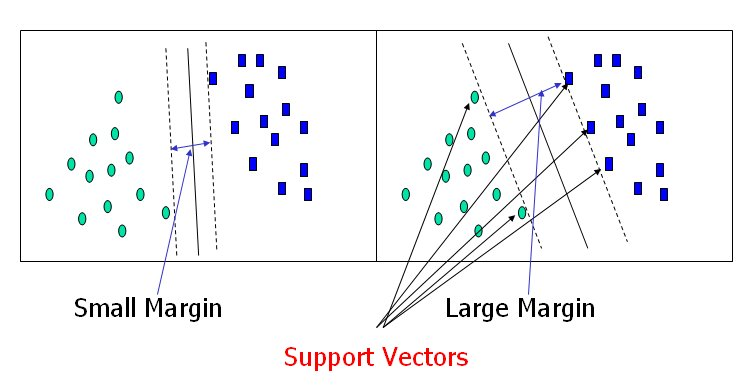
\includegraphics[width=\textwidth]{Figures/svm}
\decoRule
\caption[Support Vector Machines]{Support vector machines with their support vectors. \cite{svm}}
\label{fig:svm}
\end{figure}

\subsection{Linear and non-linear classifiers}
\label{linearclass}
\noindent Normally Support Vector Machines, as well as general logistic regression work with linear classifiers. A classifier can be linear or non-linear. A linear classifier has a decision boundary which is a linear function. This can be visualised by visualising that there is a line drawn through the data. On one side of this line, the data belongs to one class. Data on the other side of this line belongs to another class. \cite{linearClassifier} \\
\\
Sometimes problems cannot be solved with linear classifiers. When training data contains a lot of noise for example. Noise in data could mislead the learning method and increase the classification error. Figure~\ref{fig:linearvsNonLinearClassifier} shows classification of webpages being Chinese or English web pages. This seems to be a linear problem and a linear classifier has divided the space in the two classes (dashed line and short dashes). However, there are three noise documents (marked with arrows). The noise is misleading the classifier. It increases the classification error. \cite{linearvsNonLinearClassifier} \\
\\
However, when a non-linear classifier is applied, the noise is not a problem anymore. The noise elements belong to their respective classes. This classifier performs better than the linear classifier. In this example, the noise elements are considered important and that has as effect that the non-linear classifier is not considered overfitted. \cite{linearvsNonLinearClassifier}

\begin{figure}[H]
\centering
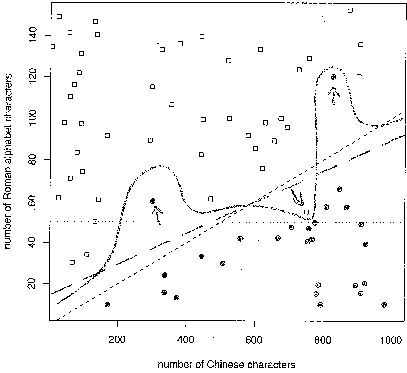
\includegraphics[width=0.8\textwidth]{Figures/classifierNoise}
\decoRule
\caption[Linear and non-linear classifiers]{Linear and non-linear classifiers. \cite{linearvsNonLinearClassifier}}
\label{fig:linearvsNonLinearClassifier}
\end{figure}

\subsection{Kernels}
\label{kernels}
 In order to adapt Support Vector Machines to be able to fit non-linear classifiers, some adjustments need to be done. This can be done with kernels. A kernel is a similarity or inverse distance function. Which can be any of the functions seen in Section~\ref{distancemetric}. The function compares two inputs (data points) and computes their similarity. The more similar two data points are, the smaller the distance in between them. This means that there is an inverse relation between distance metrics and kernels. \\
\\
Using a kernel in Support Vector Machines, rather than preprocessing the entire feature space, all features at once, is called the kernel trick. \cite{kernelTrick}. \\
\\
The kernel trick is often computationally cheaper than the explicit computation of "new" features which represent data and their similarity. Normally features are extracted from data and then fed into a machine learning algorithm. Kernels offer an alternative. \\
\\
The kernel should be a function to compare input data. The kernel, along with labeled data is then used to construct features. In literature, when no special kernel is used, the algorithm is said to use a linear kernel. One of the most basic kernels is just using a simple distance metric. This could be the inverse of the Euclidean distance as seen in Section~\ref{distancemetric}.\\
\\
A more advanced type of kernels are called Gaussian (or RBF) kernels. Gaussian kernels are also one of the most popular type of kernels and is often used. Gaussian kernels use the squared Euclidean distance between two features. However, instead of taking the inverse of the squared Euclidean distance, it uses the exponential function. The exponent is the negative of the squared Euclidean distance. 

\section{K-Nearest Neighbors}
\label{algorithm:knn}
The K-Nearest Neighbors or KNN algorithm is a supervised learning algorithm which computes the classification by looking at the classes of the K-Nearest neighbors of the training data. The K-Nearest Neighbors is an Instance-based algorithm. \cite{mlcat} The chosen class is the class most common among its K-Nearest neighbors, this can be seen in Figure~\ref{fig:knn}. K is typically a small number. When K is equal to 1, the assigned class is the same as the class of the closest sample. 

\begin{figure}[H]
\centering
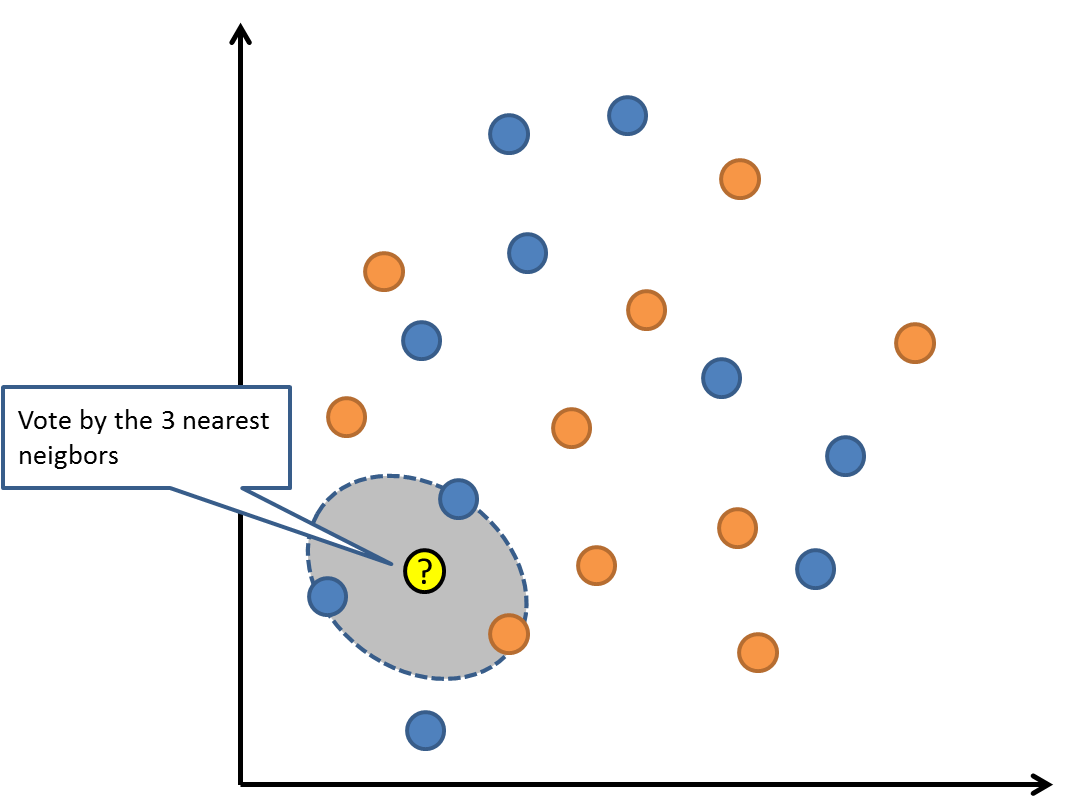
\includegraphics[width=0.8\textwidth]{Figures/knn}
\decoRule
\caption[K-Nearest Neighbors]{K-Nearest Neighbors. \cite{knn}}
\label{fig:knn}
\end{figure}

\noindent When training the algorithm, the input data and classes are stored. There are mutliple methods to compute the distance between data. Euclidean distance can be used for continuous data. For discrete variables another metric can be used, such as the Hamming distance. There are many different methods for computing the distance, these are explained in Section~\ref{distancemetric}.

\subsection{KNN drawbacks \& solutions}
\label{knn:sol}
\noindent A major drawback of the KNN algorithm is the weakness to skewed data. Skewed data is data that belongs to a class that is underrepresented in the complete data set. Since the class is chosen based on the most popular nearest class, these popular classes may dominate the prediction. One simple solution is to gather more data. More realistically, the problem can be overcome by taking the distance between the input data and the neighbors into account. If this does not work, it is possible to use learning algorithms to select the best data from the data set so that no class is underrepresented. These methods are far more advanced and have a higher computational cost. \\
\\
In Figure~\ref{fig:knnExample}, an example is shown with 3-class classification. In the this example, the weights are uniform. The score that decides which class is going to be predicted is computed from a majority vote. The example from Figure~\ref{fig:knnExample2} assigns weights proportional to the inverse of the distance between the data point which is being predicted and any $k$ neighbors. The distance function used to select the class is similar to $ \dfrac{1}{\text{distance between x and y}} $ with $x$ the data point for which a class is going to be predicted and $y$ a neighbor of $x$. This is the method to address skewed data. \\
\\
If $k$ would be set to $2$, then the $2$ closest neighbors are chosen. The class is then chosen based on the inverse distance. Assume that the $2$ closest neighbors belong to classes $A$ and $B$. The first neighbors is closer to the data point for which a class is going to be predicted. Then the class that is chosen for the data point is $A$, not $B$. In Figure~\ref{fig:inverse}, it can be seen that when the distance (red line) increases, the weight decreases (blue line). All weights that belong to neighbors of the same class are added together, the class with the highest score is chosen.
\begin{figure}[H]
\centering
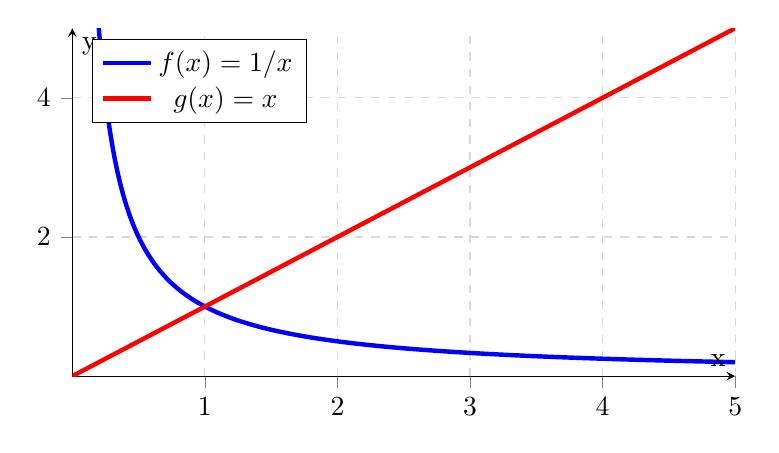
\begin{tikzpicture}
    \begin{axis}[
    	legend pos=north west,
        axis x line=middle,
        axis y line=middle,
        grid = major,
        width=10cm,
        height=6cm,
        grid style={dashed, gray!30},
        xmin=0,     % start the diagram at this x-coordinate
        xmax= 5,    % end   the diagram at this x-coordinate
        ymin= 0,     % start the diagram at this y-coordinate
        ymax= 5,   % end   the diagram at this y-coordinate
        %axis background/.style={fill=white},
        xlabel=x,
        ylabel=y,
        tick align=outside,
        enlargelimits=false]
      % plot the stirling-formulae
      \addplot[domain=0:5, blue, ultra thick,samples=500] {1/x};
      \addlegendentry{$f(x)=1/x$}
      \addplot[domain=0:5, red, ultra thick,samples=500] {x};
      \addlegendentry{$g(x)=x$}
    \end{axis}
\end{tikzpicture}
\caption{Inverse distance function} \label{fig:inverse}
\end{figure}

\begin{figure}[H]
\centering
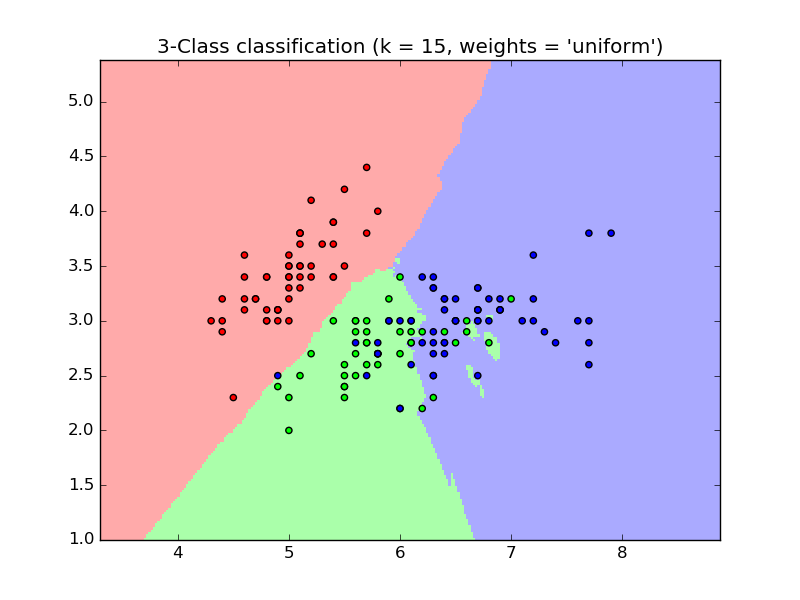
\includegraphics[width=0.7\textwidth]{Figures/knnExample}
\decoRule
\caption[K-Nearest Neighbors: Uniform weights]{K-Nearest Neighbors example with 3 classes with uniform weights. \cite{knnExample}}
\label{fig:knnExample}
\end{figure}

\begin{figure}[H]
\centering
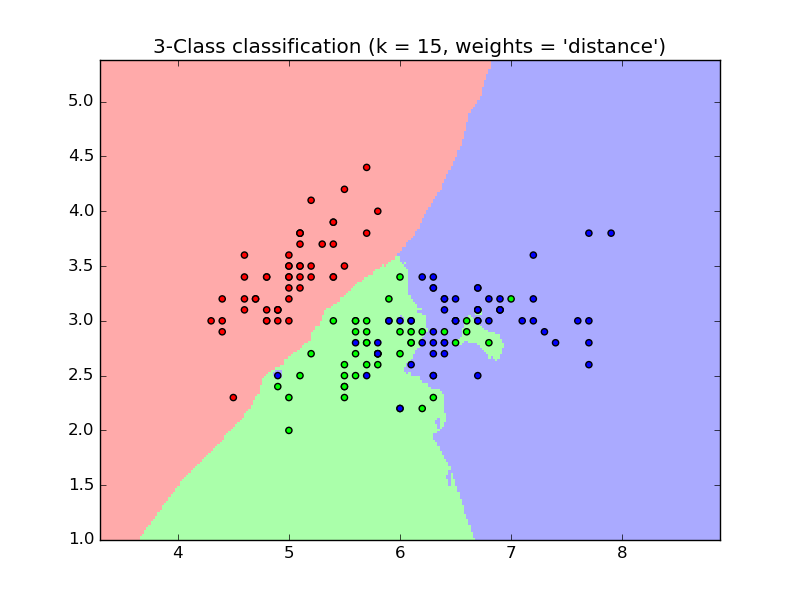
\includegraphics[width=0.7\textwidth]{Figures/knnExample2}
\decoRule
\caption[K-Nearest Neighbors: Inverse distance weights]{K-Nearest Neighbors example with 3 classes with inverse distance weights. \cite{knnExample}}
\label{fig:knnExample2}
\end{figure}


\subsection{Selection of parameter}
The best choice of $k$ depends on the problem that is being solved and on the data that is being used to learn from. Larger values for $k$ reduce the effect of noise data during prediction. However, the other effect of large values of $k$ is that classes will have less distinct bounderies between them. \\\\
In general, the presence of noise severely limits the accuracy of the algorithm. Another issue that can limit the accuracy of the algorithm is irrelevant features. There are different methods to select and scale features in order to improve accuracy. One approach is to use evolutionary algorithms. \cite{knnEvolutionary}

\section{Clustering}
Clustering is a machine learning concept using unsupervised learning. Unsupervised learning does not have labels with the training set. An unsupervised machine learning algorithm tries to find structure within the given training set. Clustering is the first type of unsupervised learning. It tries to cluster the training samples into different clusters.

\subsection{K-means Algorithm}
The K-means algorithm is a simple clustering algorithm. K is the number of clusters that is going to be used. An example of how K-means could cluster data is shown in Figure~\ref{fig:kmeansExample}. The algorithm first randomly places the K clusters in the space (from the training set). This can be done by randomly chosing K training samples. Then it repeats the following steps until the cluster centers remain stationary. it iterates over all training samples, and assigns them to the closest cluster. Next the cluster centers are moved to the center of the total cluster. \cite{kmeans2} \\
\\
\begin{python}
# choose k random samples
c = choose_random_samples(k)
do:
    for sample in all_samples:
        c_i = closest_cluster_to(sample)
        c_i.append(sample)
    c.recalculate_center()
while cluster_center_changed(c)
\end{python}~\\
The final clusters that are found by K-means are dependent on the random placement of the K clusters in the beginning. It could lead to suboptimal clustering. This can be fixed by running K-means a number of times and after each iteration check the value of the cost function to find the most efficient run of K-means. 
The cost function can be described as: \cite{kmeans}
\begin{align}
J(c, \mu) = \dfrac{1}{m} \sum\limits_{i=1}^m(|| x^{(i)} - \mu^{(i)}||)^2
\end{align}
There is a similar problem with determining the amount of clusters. The same method could be used to determine the correct number of clusters. However, manually determining the number of clusters could be more time efficient. \cite{kmeans2}

\begin{figure}[H]
\centering
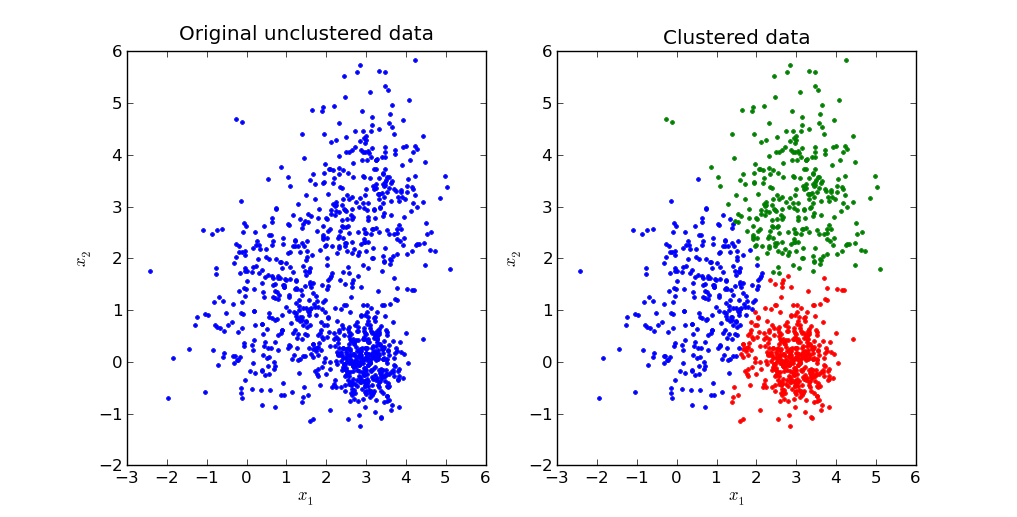
\includegraphics[width=0.9\textwidth]{Figures/kmeansExample}
\decoRule
\caption[K-means clustering]{K-means clustering. \cite{kmeansExample}}
\label{fig:kmeansExample}
\end{figure}

\section{One-class Support Vector Machine}
\label{oneclassSVM}
Support Vector Machines can also be used for unsupervised learning. The SVM will only have one class. The SVM can be trained using a dataset filled with data that belongs to that one class. The SVM learns a decision boundary around these data points as seen in the example from Figure~\ref{fig:oneclasssvmExample}. This boundary can be used to predict whether a data point belongs to that class or whether it does not. One-class SVM's can also make use of kernels.

\begin{figure}[H]
\centering
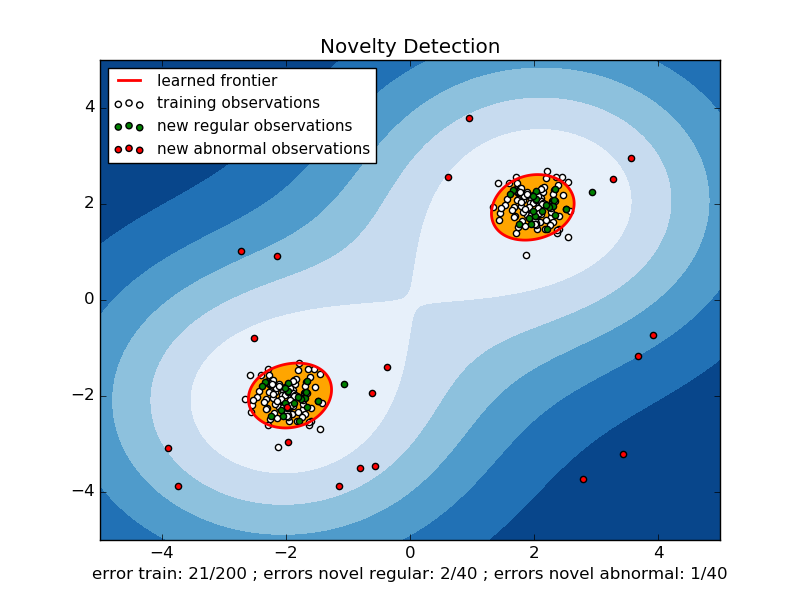
\includegraphics[width=0.8\textwidth]{Figures/oneclasssvmExample}
\decoRule
\caption[One-class SVM]{One-class SVM. \cite{oneclasssvmExample}}
\label{fig:oneclasssvmExample}
\end{figure}
 
\section{Neural networks}
\label{neuralnet}
Neural networks are a useful alternative to logistic regression if the amount of features becomes too large. The origin of neural networks are algorithms which try to mimic the brain. There is a hypothesis, the "one learning algorithm" hypothesis, that shows that the brain can learn very different things, such as sound, touch, etc. by using a single algorithm. \cite{neuralnetBrain}\\\\
A neural network is created of neurons, which are called a logistic unit. Each neuron receives input wires, and has an output wire, which computes a value using the sigmoid (logistic) hypothesis, the activation function. A neural network is a group of "neurons" that are connected together. This can be grouped into a layered approach as seen in Figure~\ref{fig:neuralnetwork}. The first layer is called the input layer, the final layer is called the output layer which outputs a $H_\theta(x)$ which is class. All layers inbetween these layers are called hidden layers. \cite{neuralnetModel1}
\begin{figure}[H]
\centering
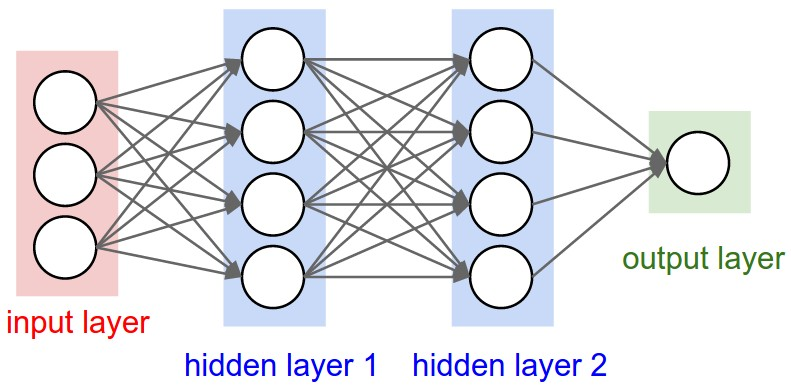
\includegraphics[width=1\textwidth]{Figures/neuralnet}
\decoRule
\caption[Neural network]{A neural network showing the different layers.\cite{neuralnetwork}}
\label{fig:neuralnetwork}
\end{figure}
\noindent Each logistic unit is denoted by $a_i^j$. $j$ is the layer and $i$ is the position in that layer. $\theta^j$ is a matrix of weights or parameters controlling function mapping from layer $j$ to layer $j+1$. $s_l$ is the number of units within a layer. The number of layers is denoted by $L$.\\\\
The neural network works similar to logistic regression, except that it performs logistic regression from layer to layer. The parameters $\theta_j$ required are learned by itself. The architecture of a neural network refers to the way the units are connected to eachother. Neural networks can be used for multi-class classification. Here, there are mutliple units in the output layer and each unit represents a different class. $K$ will denote the amount of output units. \cite{neuralnetClass}
\begin{figure}[H]
\centering
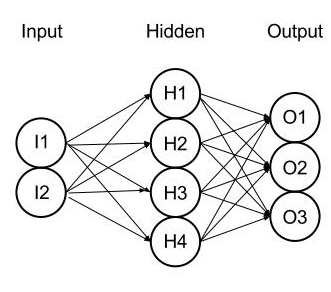
\includegraphics[width=0.7\textwidth]{Figures/neuralnetmulti}
\decoRule
\caption[Neural network with multi-class classification]{A neural network capable of multi-class classification. \cite{neuralnetworkmult}}
\label{fig:neuralnetworkmult}
\end{figure}
\noindent Data flows using the principle of forward propagation. The data passes through the first layers, moves to the second layers and so on, until it arrives at the final layer. Mathematically this can be described as: 
\begin{align*}
a^{(1)} = x\\
a^{(2)} = g( \theta^{(1)}*a^{(1)} )
\end{align*}
$a^{(1)}$ is the input layer and $x$ are the features of a data point that are fed to the neural network. $g( \theta^{(1)}*a^{(1)} )$ is the sigmoid logistic regression function with as input $\theta^{(1)}*a^{(1)}$. $\theta^{(1)}*a^{(1)}$ can be defined as $z^{(1)}$ to make the formulas simpler. This is a standard example of logistic regression. This happens for every node in a layer and for every layer. Every layer takes as input, the output from the previous layer. The data propagates forward through the network. \cite{neuralnetModel2}
\subsection{Cost function and backpropagation}
The cost function for neural networks is a generalisation of the cost function for logistic regression. The cost function accounts for the different layers, units and the number of output units. To minimize the cost function, the same methods such as gradient descent can be used. However, the problem is how to compute the partial derivative of the cost function. Using backpropagation, it is possible to compute this. \cite{neuralnetCost} \\\\
The resulting class is known in the final layer. From here, the algorithm can find the error. $\delta_j^l$ will be the symbol used for the error of node $j$ in layer $l$. \\
\\
The algorithm works backwards. It starts in the final layer. It calculates the error in this layer which is $\delta_j^{(4)} = a_j^{(4)} - y_j$ and starts working backwards. In the previous layer, the weighted sum is used of the errors from the final layer. This is $(\theta^{(3)})^T\delta^{(4)}$. This happens from layer to layer and each time, the error is calculated using the $\theta$ values from that layer.
\subsection{Using a neural network}
A neural network should have as many input units as the dimension of features. The number of output units is equal to the number of classes. Default, there should be either 1 hidden layer or if there are more, all layers should have the same number of hidden units. \cite{neuralnettraining} The neural network should be trained by first assigning random weights to the values of $\theta$. Afterwards, forward propagation should be used to get $H_\theta(x^{(i))}$. Next the cost function should be computed. Backwards propagation is used to compute the partial derivatives. The result of backwards propagation can be checked by numerical methods to compute the gradient. Finally gradient descent or other advanced optimization methods with backpropagation should be used to try to minimize the cost function as a function to the parameters $\theta$.  \\\\
A neural network could be used to implement Autonomous Driving. The neural network can be trained using images which display a road.  \cite{neuralnetDriving} The labeled data could be classes explaining whether the road goes straight,  left or right. This could be used to make vehicles drive on a road, but could also be used to program drones to be able to navigate through forest paths.  \cite{neuralnetDrone}

\subsection{Deep neural networks}
Deep Learning Algorithms are a modern modification to Artificial Neural Networks that exploit abundant cheap computation. Deep learning networks are very deep and complex neural networks. They contain a lot of hidden layers. Deep Boltzmann Machine (DBM), Deep Belief Networks (DBN) and Convolutional Neural Network (CNN) are examples of deap learning algorithms. These algorithms have specific rules aboout how the network is connected. \cite{Goodfellow-et-al-2016-Book}

\section{Decision tree algorithms}
\label{decisiontree}
Decision tree algorithms are a set of supervised learning algorithms used for classification and regression. The algorithms try to create a model that resembles a tree. Every prediction starts at the root of the tree. At every node, a certain decision rule is used. A decision rule is a condition, for example it could be: "Is feature A larger than $10$". Once a leaf of the tree is reached the correct class or value is found. \cite{decisiontree} An example of this can be seen in Figure~\ref{fig:decisiontreeExample} \\\\

\begin{figure}[H]
\centering
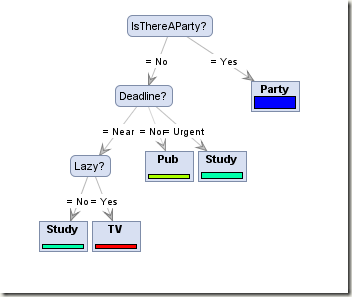
\includegraphics[width=0.7\textwidth]{Figures/decisiontreeExample}
\decoRule
\caption[Decision Tree Algorithm example]{Decision Tree Algorithm example \cite{decisiontreeExample}}
\label{fig:decisiontreeExample}
\end{figure}
\noindent Descision tree algorithms usually work top-down. They chose a feature and look through the training data to check how many children need to be made. For example, in Figure~\ref{fig:decisiontreeExample}, there is a feature "Deadline" which has $3$ different values. In this case, the tree can create $3$ children. In each child, the next feature is chosen and the process starts over until every training sample that would end up in this spot, all belong to the same class. When features are continuous, the algorithm tries to find ways to distinguish certain values. For example, for one feature, half of all training samples are larger than $100$, the other half is smaller than $100$. Then a check: "Is this feature larger or smaller than $100$" might be chosen. \\
\\
\noindent A decision tree is simple to understand and to visualise. They are also quite fast. However, a decision tree algortihm can easily create complex trees and overfit. They also cannot handle skewed data that well. \cite{decisiontree}

\section{Bayesian Algorithms}
\label{bayesalg}
There are Bayesian Algorithms which explicitly apply Bayes’ Theorem for problems such as classification and regression.There are a lot of variances on Bayesian Algorithms, the most popular is Naive Bayes. \cite{mlcat} Naive Bayes is decent for classification but is not optimal for regression. \cite{naivebayes} \\\\
Bayes Theorem is stated as follows \cite{bayes}:
\begin{align}
P(A|B) = \dfrac{P(B|A) * P(A)}{P(B)}
\end{align}
$A$ and $B$ are events. $P(A)$ is the chance that event $A$ happens and $P(B)$ is the chance that event $B$ happens. $P(A | B)$, a conditional probability, is the probability of event $A$ given that $B$ is true.  $P(B | A)$ is the probability of event $B$ given that $A$ is true. \cite{bayes} \\\\
Naive Bayes is a supervised learning algorithm with the "naive" assumption that every feature is independent. The formula for the Bayes' Theorem is used for Naive Bayes. The event $A$ is a class. $B$ is the collection of features. \cite{naivebayes} \\
\\
In the Naive Bayes algorithm, for every class, the probability is calculated that that class belongs to the given sample for which a class is being predicted. The probability is: $P(class | x_0, x_1, ..., x_n)$. For this formula, the Bayes's Theorem can be applied. $P(x_0, x_1, ..., x_n)$ is constant since it only depends on the features. $P(x_0, x_1, ..., x_n | class)$ can be written as $P(x_0 | class) * p(x_1 | class) * ... * p(x_n | class)$ because of the naive assumption. All of these can be found during the training phase. \\
\\
When training, $P(class)$ is the fraction of how much the class is represented in the training data.\\ $P(x_i | class_j)$ for every feature can be found by looking at the training samples and looking at how much $x_i$ is represented when the class is $class_j$. When $x_i$ is not present in the training set, the distribution of the different values for $x_i$ are used to find out how much $x_i$ could be represented.

\section{Association Rule Learning Algorithms}
Association Rule Learning Algorithms are methods that extract rules that best explain observed relationships between variables in data. Apriori algorithm and Eclat algorithm are examples of such algorithms. These algorithms operate mainly on databases.   \cite{mlcat} \\\\
In Figure~\ref{fig:apriori}, an example is given of a small database. Association Rule Learning could make several rules from this database. A rule could be "if a set contains alpha and beta, then there is a 50\% chance that it also contains epsilon". \cite{apriori} It does this by counting items. First it counts the frequency that alpha, beta, etc. appears in the database. Next, it counts the all the pairs $(alpha, beta)$. The algorithm continues until it cannot make any more sets. From these sets, it can make the association rules. 

\begin{figure}[H]
\centering
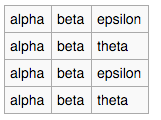
\includegraphics[width=0.7\textwidth]{Figures/Apriori}
\decoRule
\caption[Apriori Algorithm example]{Apriori Algorithm example \cite{apriori}}
\label{fig:apriori}
\end{figure}

\section{Specific algorithms for a sub-field}
A lot of algorithms are specifically constructed for a specific sub-field of machine learning, for example computer vision, natural language processing, etc. Even within the categories of algorithms that were discussed, regression, regularization, instance-based, clustering and neural networks, there are a lot of different variants. However, these are considered to be to advanced and outside of the scope of this thesis. 
